\clearpage
\subsection{Procedure Call} % (fold)
\label{sub:procedure call}

A procedure call is a kind of \nameref{sub:statement} that instructs the computer to run the code in a \nameref{sub:procedure}. This statement uses the procedure's name to identify the procedure that must be run. If the procedure called requires some data, this data is \emph{passed} to the procedure as part of the procedure call.

\begin{figure}[h]
   \centering
   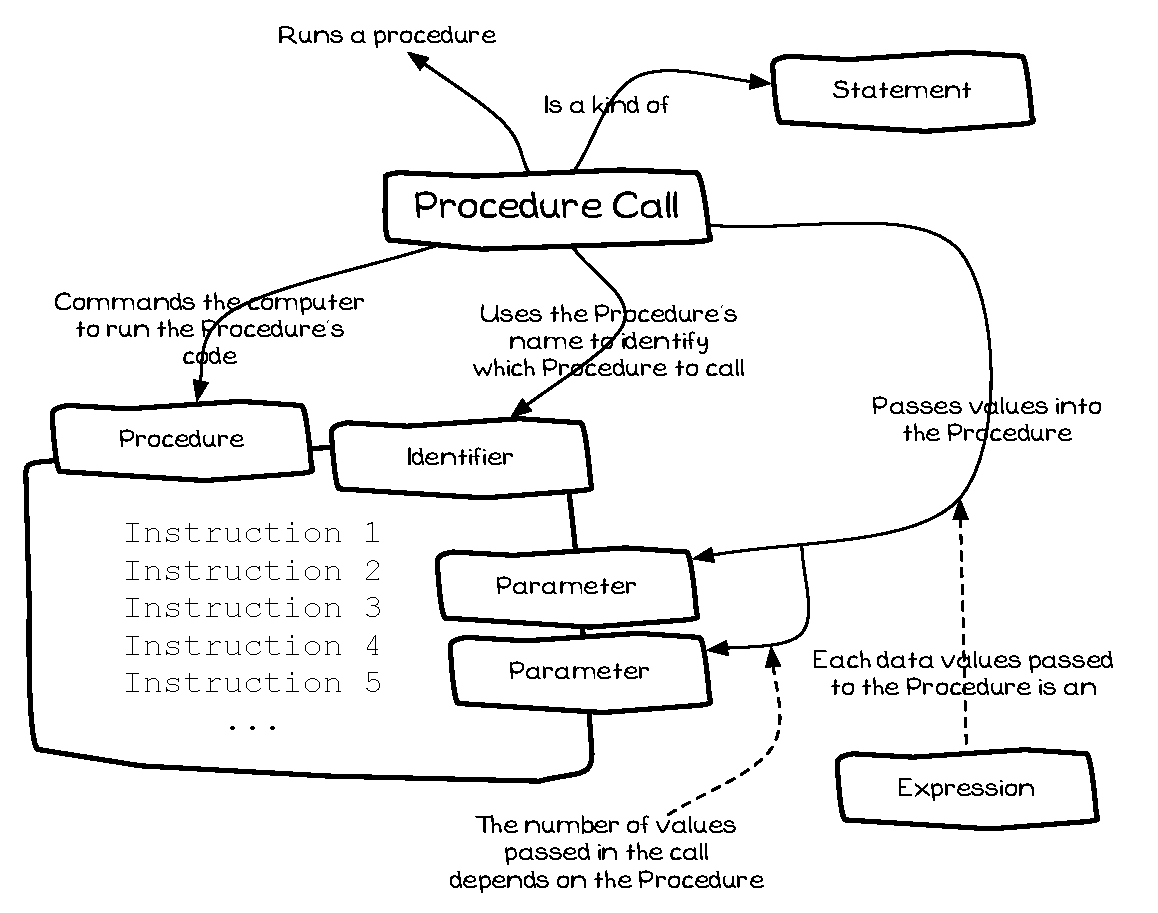
\includegraphics[width=\textwidth]{./topics/program-creation/diagrams/ProcedureCall} 
   \caption{A procedure calls runs a procedure, passing in values for the procedure to use}
   \label{fig:program-creation-procedure call}
\end{figure}


\mynote{
\begin{itemize}
  \item A procedure call is an \textbf{action}, you can call procedures in your code.
  \item Figure \ref{fig:program-creation-procedure call} shows the concepts related to the procedure call.
  \item A procedure call is an instruction to execute a procedure.
  \item You can code a procedure anywhere you can code a statement.
  \item The \nameref{sub:identifier} indicates the \nameref{sub:procedure} to run.
  \item Data values passed to the procedure are coded using \nameref{sub:expression}s.
  \item When the procedure's task is complete the program continues with the next \nameref{sub:statement}.
\end{itemize}
}

% section program (end)